\chapter{The Finished Application}
INTROTEXT TO CHAPTER
\section{The iOS Application}

The application is build for iOS using Xcode and Swift 4.0. The app has been developed specifically for iPhone X. It has also only been tested on iPhone X. However, the app should work on other iPhone models that support ARKit 2.0 as well.

\subsection{Class diagrams}
Below are some class diagrams for the reader to better understand what different parts there are, 
how they fit together and how the application works as a whole. The diagrams are divided into 
three parts to be readable in the paper.

\begin{figure}[!hbtp]
\begin{center}
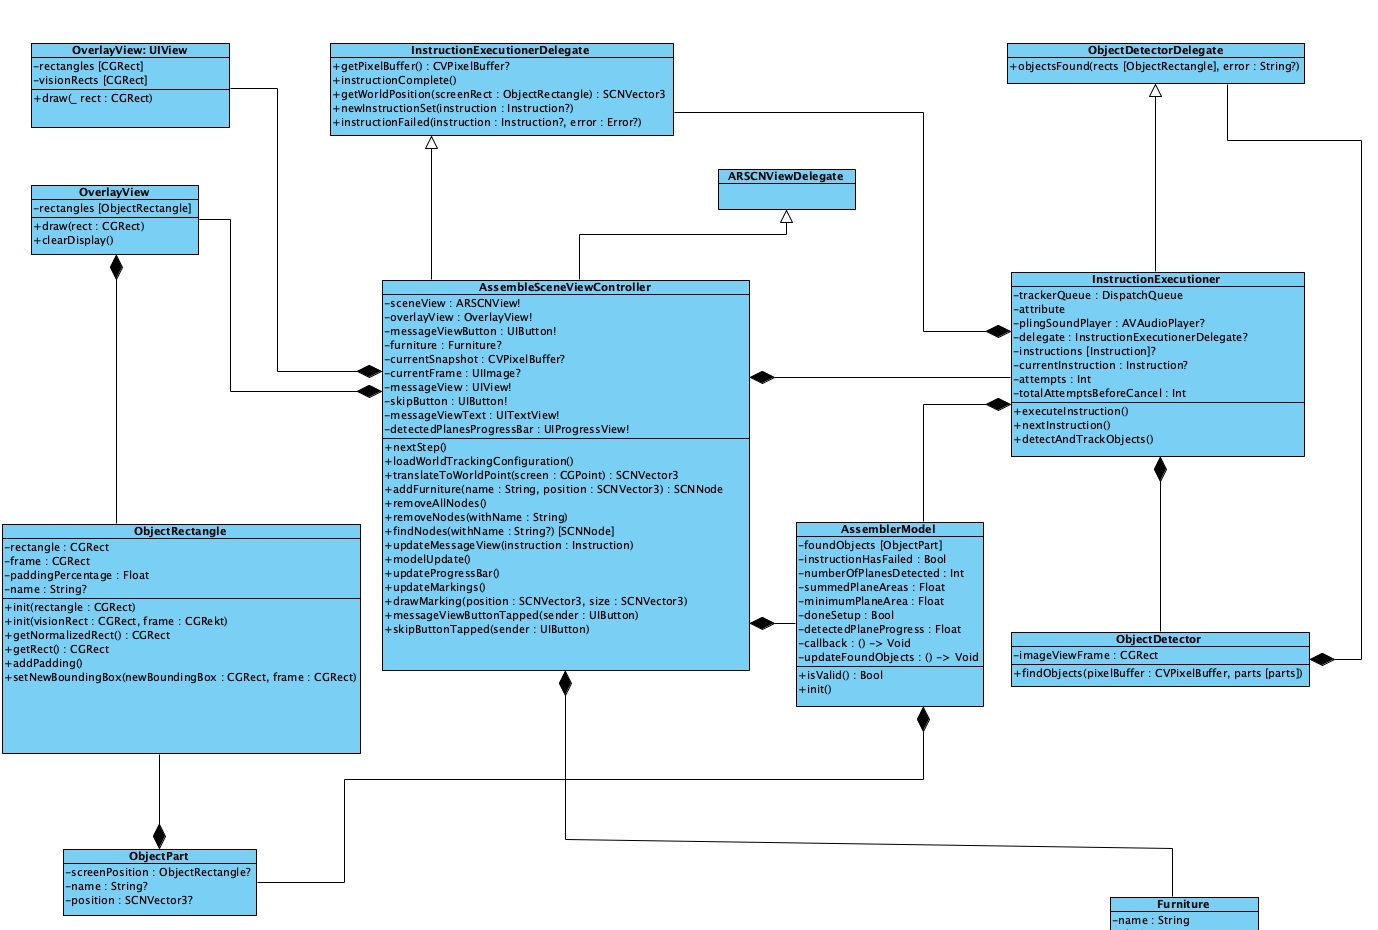
\includegraphics[width = 1.1\textwidth]{./Images/AssemblerClassDiagram1.jpg}
\caption{A class diagram of the assembler view part of the application. The Furniture class in the lower right is incomplete and is shown in the next diagram.}
\label{fig:classdiagramassembler}
\end{center}
\end{figure}

The application follows the Model View Controller design pattern as well as the Delegate design pattern.
This decision was made since many tools and features in iOS and Swift are implemented that way,
so we are just following the standard procedure.

\textbf{AssemblerViewController} is the controller for the view that holds the ARSCNView.
It is responsible for what happens when the user taps on a button in that view and displaying the correct
information to the user at the right times. It also holds the \textbf{Instruction Executioner} which holds a 
set of instructions that it gets at initialisation. The instruction executioner executes the current
instruction and therefore decides what will happen when it executes. Every instruction is executed on a worker queue thread to avoid the video feedback to freeze during execution.\\

The InstructionExecutioner holds the \textbf{ObjectDetector} which finds specific objects in a 
trained model from a pixel buffer. The found objects are passed back as \textbf{ObjectRectangles} through the delegate. The object rectangles are bounding boxes
of the objects on screen. They are represented as CGRect's and can be stored and fetched as
either regular or normalized rectangles. The normalized variants are needed in all kinds of machine learning purposes and the regular form are used in all GUI purposes, such as in the \textbf{OverlayView}. (Normalized 
rectangles have values of 0-1 for widths, heights, x-, and y-position. The origin is in the lower left 
corner.)\\

The \textbf{AssemblerModel} is the model in the AssemblerViewController, but is also used in the InstructionExecutioner since they are highly dependent on each other.
The most important attributes it holds are the \textbf{ObjectParts} that have been spotted by the 
app during the execution of the current instruction.
That way, all the parts needed for the current instruction do not need to be in the same image 
together but instead can be spotted separately.\\

\begin{figure}[!hbtp]
\begin{center}
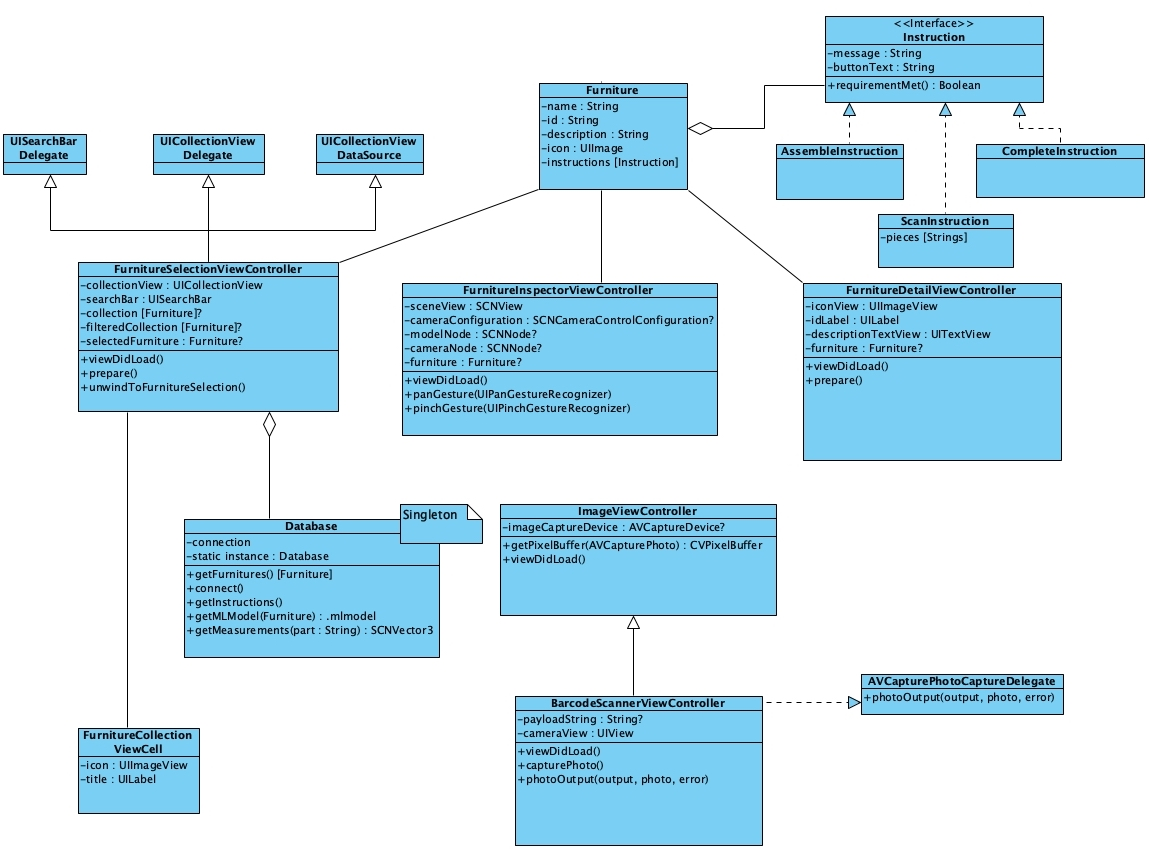
\includegraphics[width = 0.9\textwidth]{./Images/FurnitureClassDiagram.jpg}
\caption{A class diagram of the furniture selection views part of the application. The Furniture class.}
\label{fig:classdiagramassembler}
\end{center}
\end{figure}

The furniture that the user wants to put together is selected in a collection view \textbf{FurnitureSelectionViewController}
which conforms to the UICollectionViewDelegate- and UICollectionViewDataSource protocol for the collection view functionality.
The data to be viewed in the controller is fetched from the \textbf{Database} class.
The return data from the class are hardcoded from the start but can easily be changed to fetch
data from a server.\\

The \textbf{Furniture} holds all the information about a specific furniture as well as the instruction set of how to put it together. The instruction set consists of \textbf{Instruction}'s that can be
of the kind \textbf{ScanInstruction}, \textbf{AssembleInstruction} or \textbf{CompleteInstruction}.
A regular Instruction is usually just text instructions to the user, while the scan instructions tell the instruction executioner to look for specific parts during that step.
The assemble instruction is run when the user is in the process of assembling two parts.
Finally the complete instruction is given which tells the executioner that the furniture has been fully assembled.\\

For scanning barcodes, the \textbf{BarcodeScannerViewController} is used, which inherits all the photo capture functionality from the \textbf{ImageViewController}.\\

\begin{figure}[!hbtp]
\begin{center}
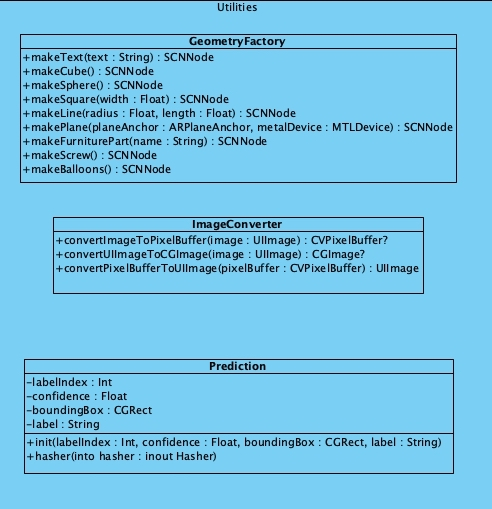
\includegraphics[width = 0.5\textwidth]{./Images/UtilitiesClassDiagram.jpg}
\caption{A class diagram of the utilities part of the application. These are some classes that make the rest of the code in the application easier to understand and use.}
\label{fig:classdiagramassembler}
\end{center}
\end{figure}

In the utilities folder there are some classes that simplifies the rest of the application
by holding code that removes a lot of redundancy.

The \textbf{GeometryFactory} creates all the 3D geometry for the ARScene and return the nodes 
containing this geometry. An example is that it can create all the furniture parts as virtual object 
nodes to be placed in the scene.

A lot of conversion between pixel buffers and UIImage's are made and the \textbf{ImageConverter }
eases the pain of having to do that in many places.

Finally the \textbf{Prediction} class helps the object detector when getting results
from the VNCoreMLRequest.

\subsection{Connecting two pieces in AR}
After finding the specific pieces that are supposed to be connected they are created as
virtual objects in the scene on their respective locations. The location is determined using
hit tests of the screen positions to the detected plane from the ARScene.

The virtual objects are rendered in the scene using SCNNode's as talked about in \ref{subsecARKit} and the node position is the origin of the 3D model. The origin has been chosen to be at a location that is touching the floor when it is standing. That way they can easily be placed to look like they are standing right on the floor.
When both pieces are placed in the scene they are to be moved with an animation in a way so that they become connected.

Each virtual object node can embed another node called the "anchor point". The position of this node within the parent node is where the other object is to be connected. To connect them, either the object without the anchor point moves to the anchor point position, or the two object move so that each of their anchor points are at the same position.
This is accomplished using the algorithm below.

\begin{lstlisting}[language=swift]
    var furniturePartNodes = [SCNNode]()

        for object in model.foundObjects
        {
            guard object.name != nil else { return }
            guard object.position != nil else { return }
            
            let furnitureNode = addFurniture(part: object.name!, position: object.position!)
            furniturePartNodes.append(furnitureNode)
        }
        
        var previousNode: SCNNode? = nil
        var previousAnchorPoint: SCNNode? = nil
        
        var nodeActions = [(SCNNode, [SCNAction])]() // A list for storing animations to run on a node later
        
        for node in furniturePartNodes
        {
            var actions: [SCNAction] = []
            actions.append(SCNAction.rotate(by: -CGFloat.pi / 2, around: SCNVector3(0, 0, 1), duration: 1))

            let anchorPoint = node.childNode(withName: ANCHOR_POINT, recursively: true)
            
            if anchorPoint == nil
            {
                if previousAnchorPoint != nil
                {
                    actions.append(SCNAction.move(to: previousAnchorPoint!.worldPosition, duration: 2))
                }

                previousNode = node
            }
            else
            {
                previousNode?.runAction(SCNAction.move(to: anchorPoint!.worldPosition, duration: 2))
                if previousAnchorPoint != nil
                {
                    actions.append(SCNAction.move(to: previousAnchorPoint!.worldPosition, duration: 2))
                    actions.append(SCNAction.move(by: node.worldPosition.substract(other: anchorPoint!.worldPosition), duration: 2))
                }

                previousAnchorPoint = anchorPoint
            }
            
            // HACK: Adds an extra action with no content at the end to make completion handler wait until the last action is done
            actions.append(SCNAction.move(by: SCNVector3Zero, duration: 1))
            
            nodeActions.append((node, actions))
        }
}
\end{lstlisting}

Afterwards, the items in 'action' are performed on the respective node.

\subsection{The finished GUI}
The finished GUI is similar to the prototype but some details are different.

\begin{figure}[!hbtp]
\begin{center}
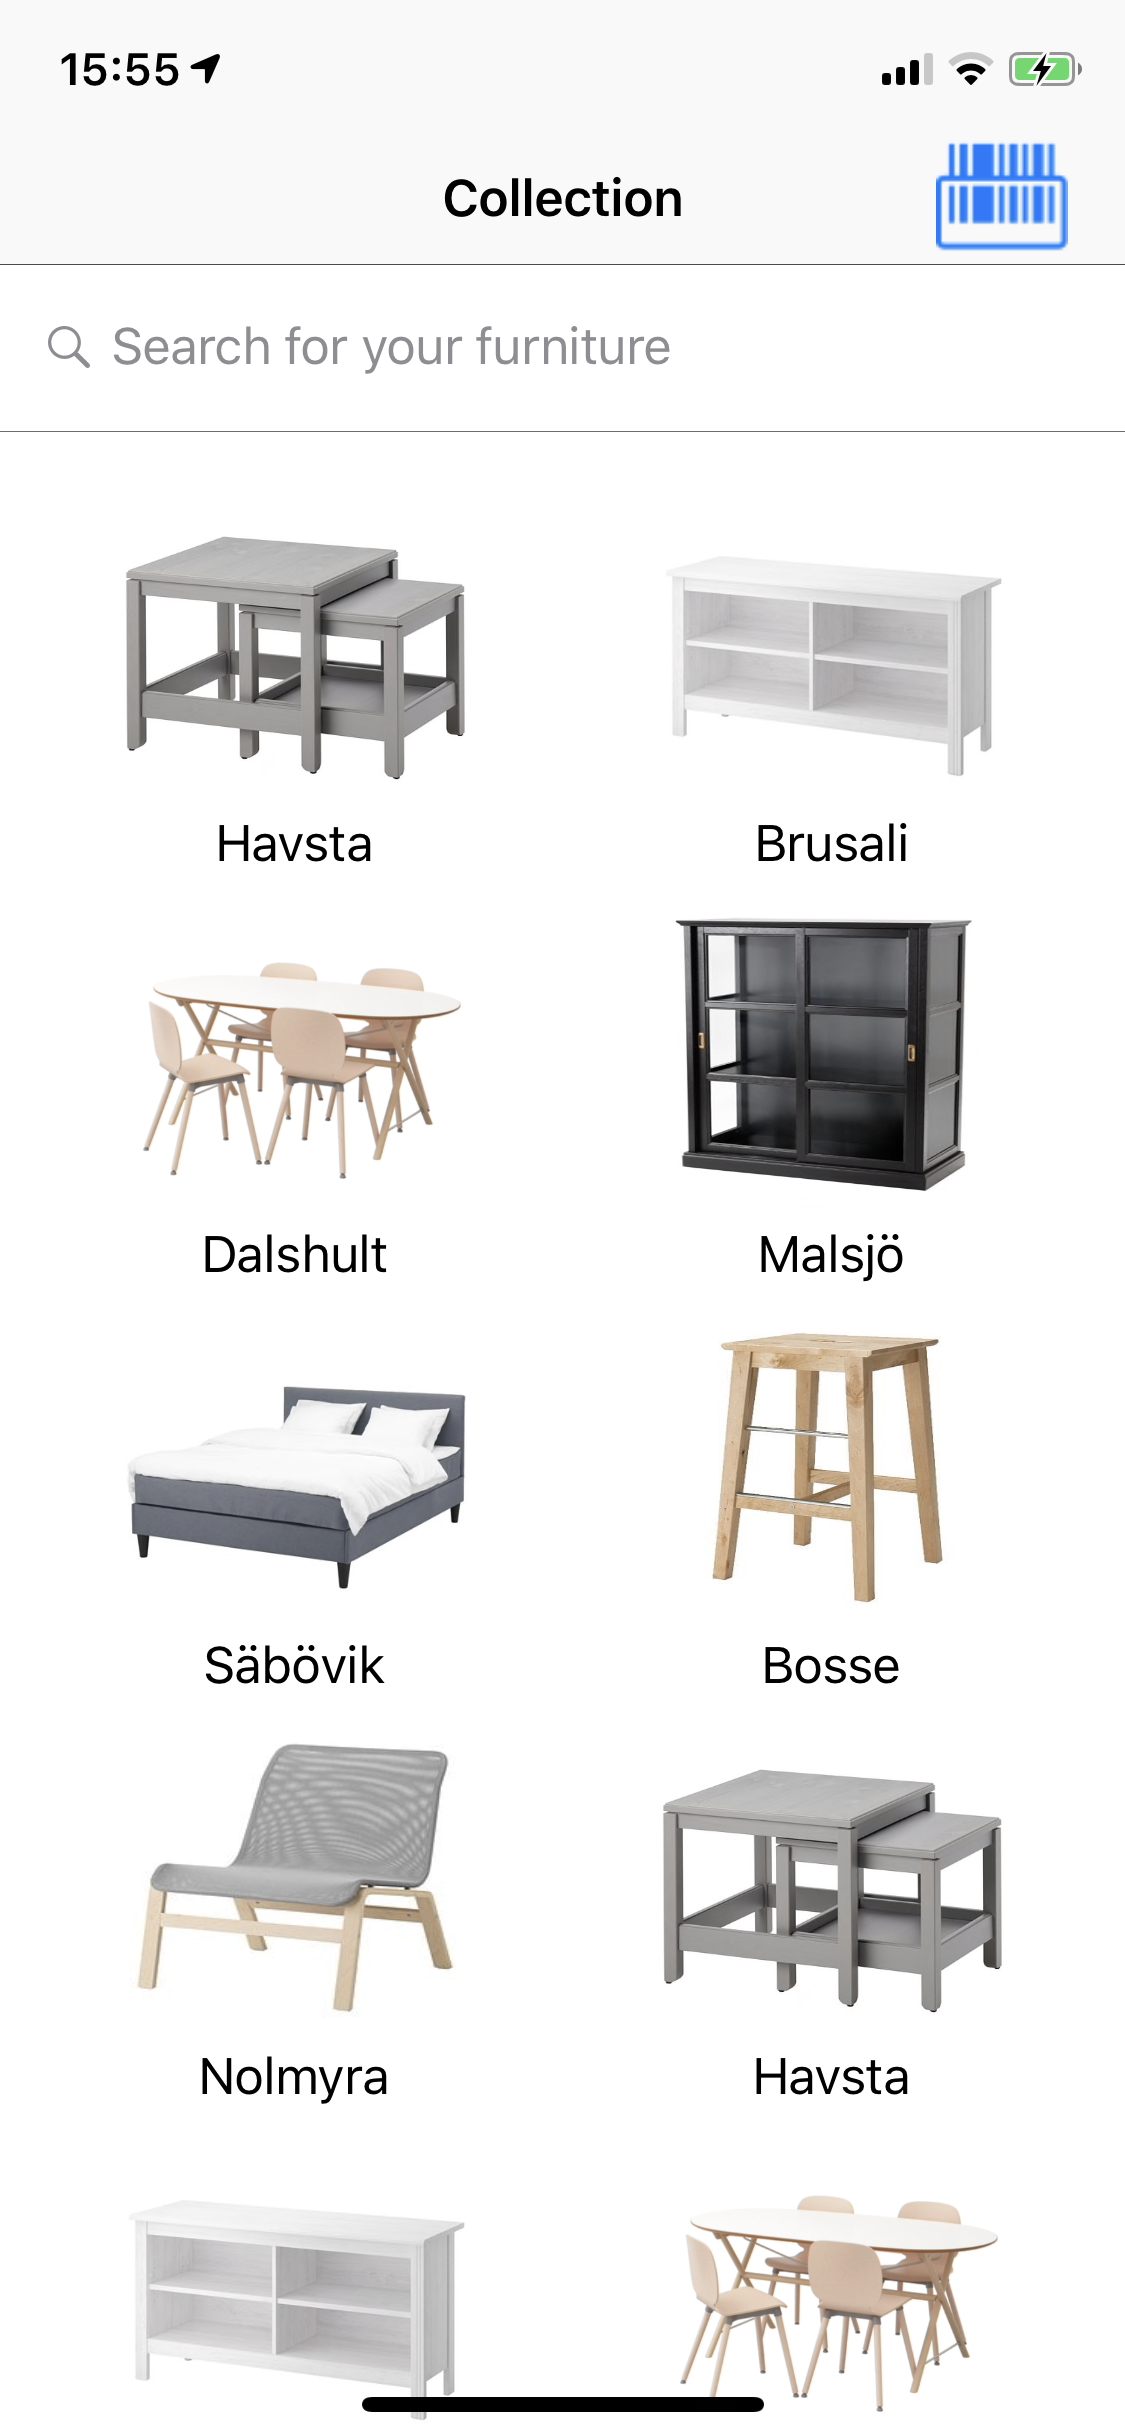
\includegraphics[width = 0.3\textwidth]{./Images/Application1}
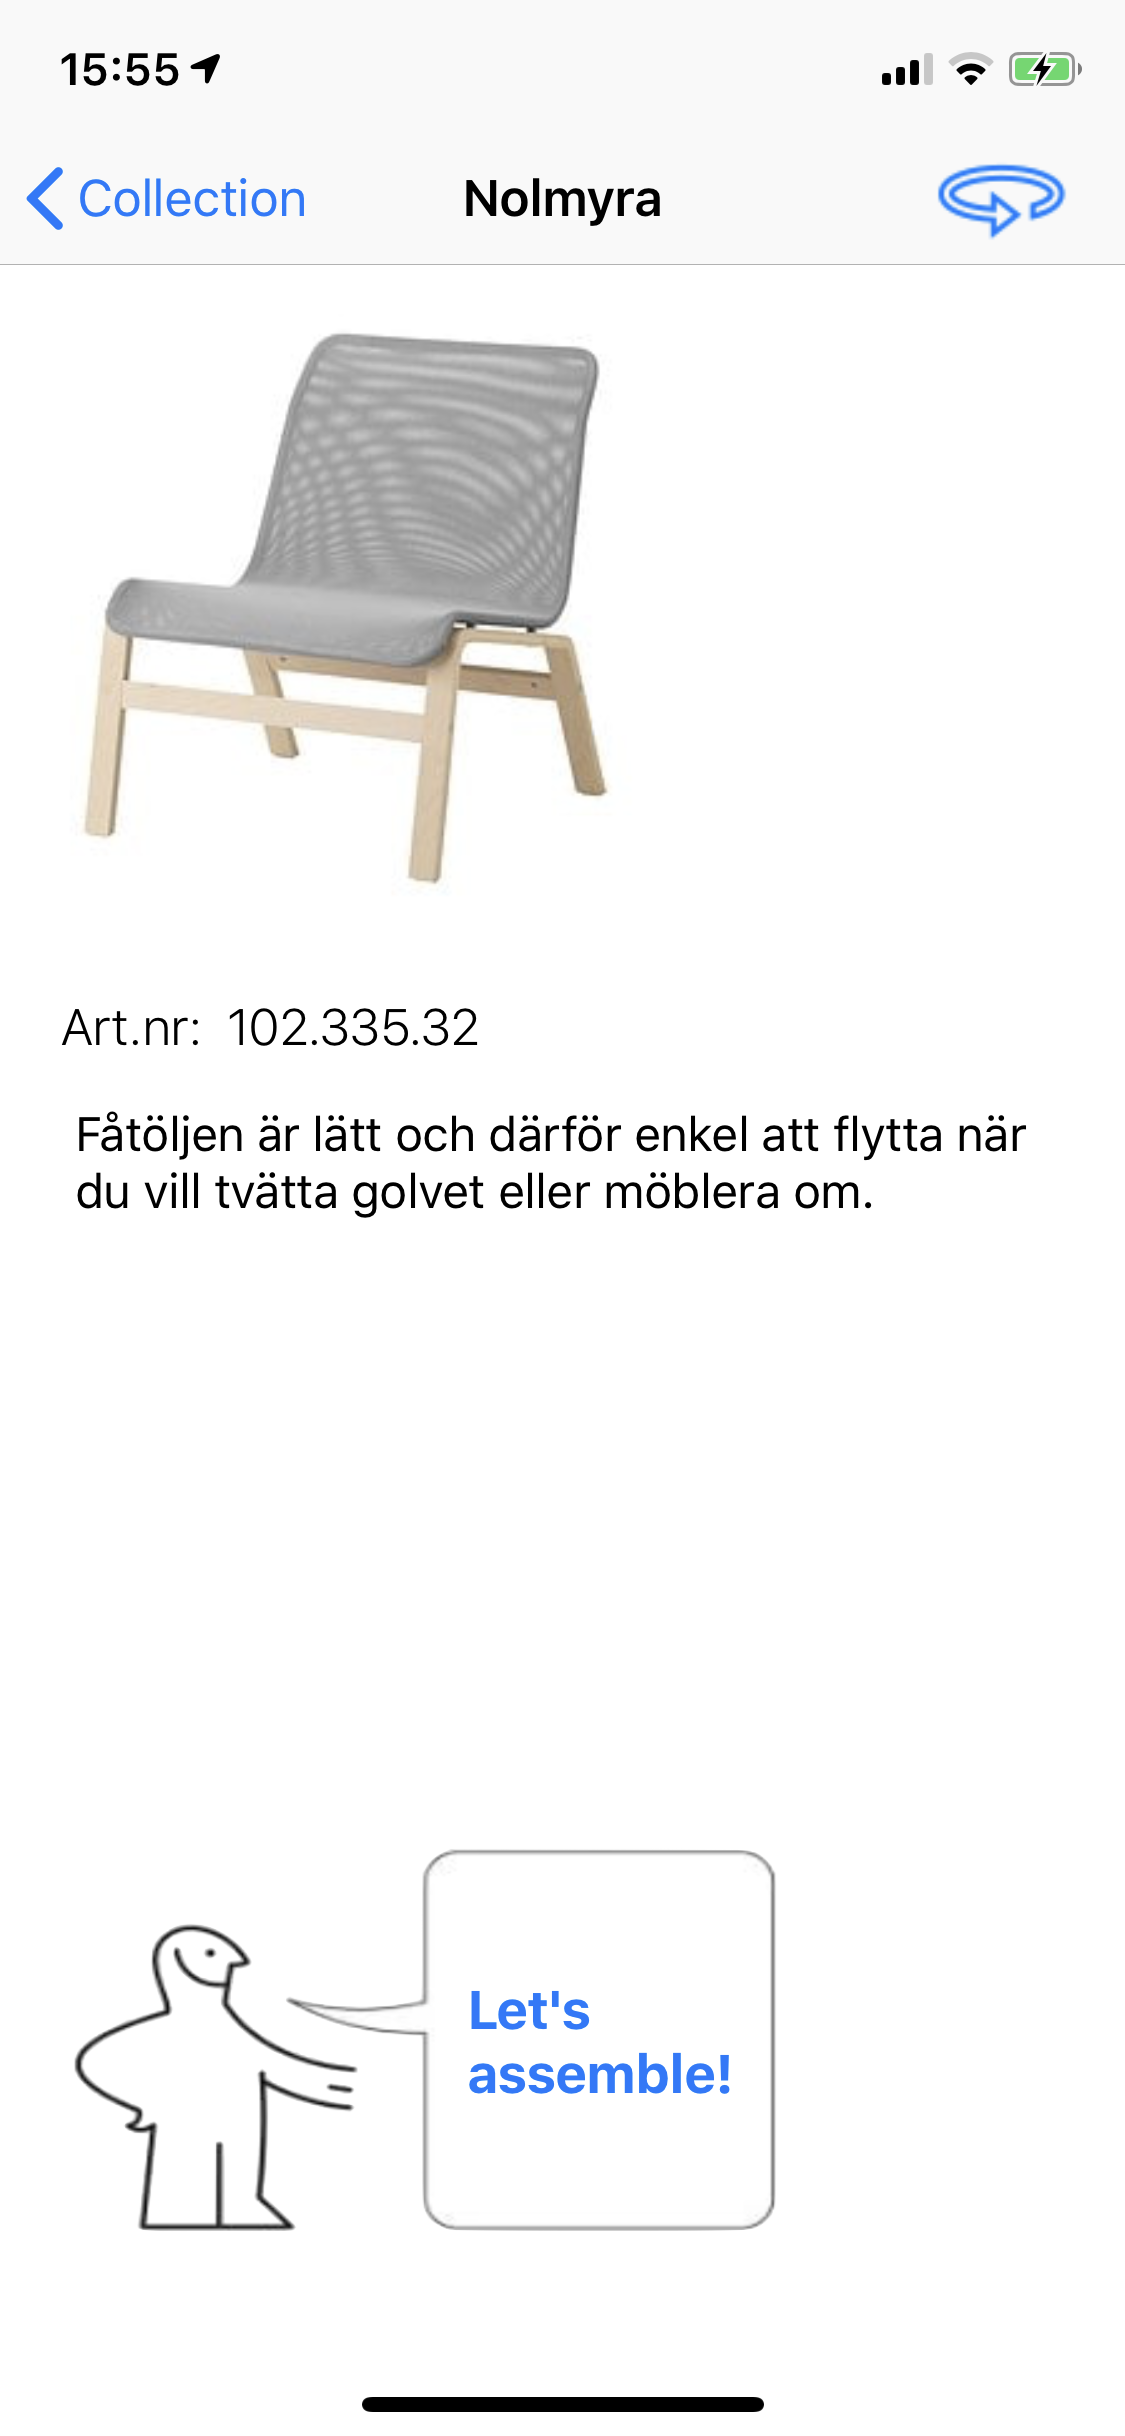
\includegraphics[width = 0.3\textwidth]{./Images/Application2}
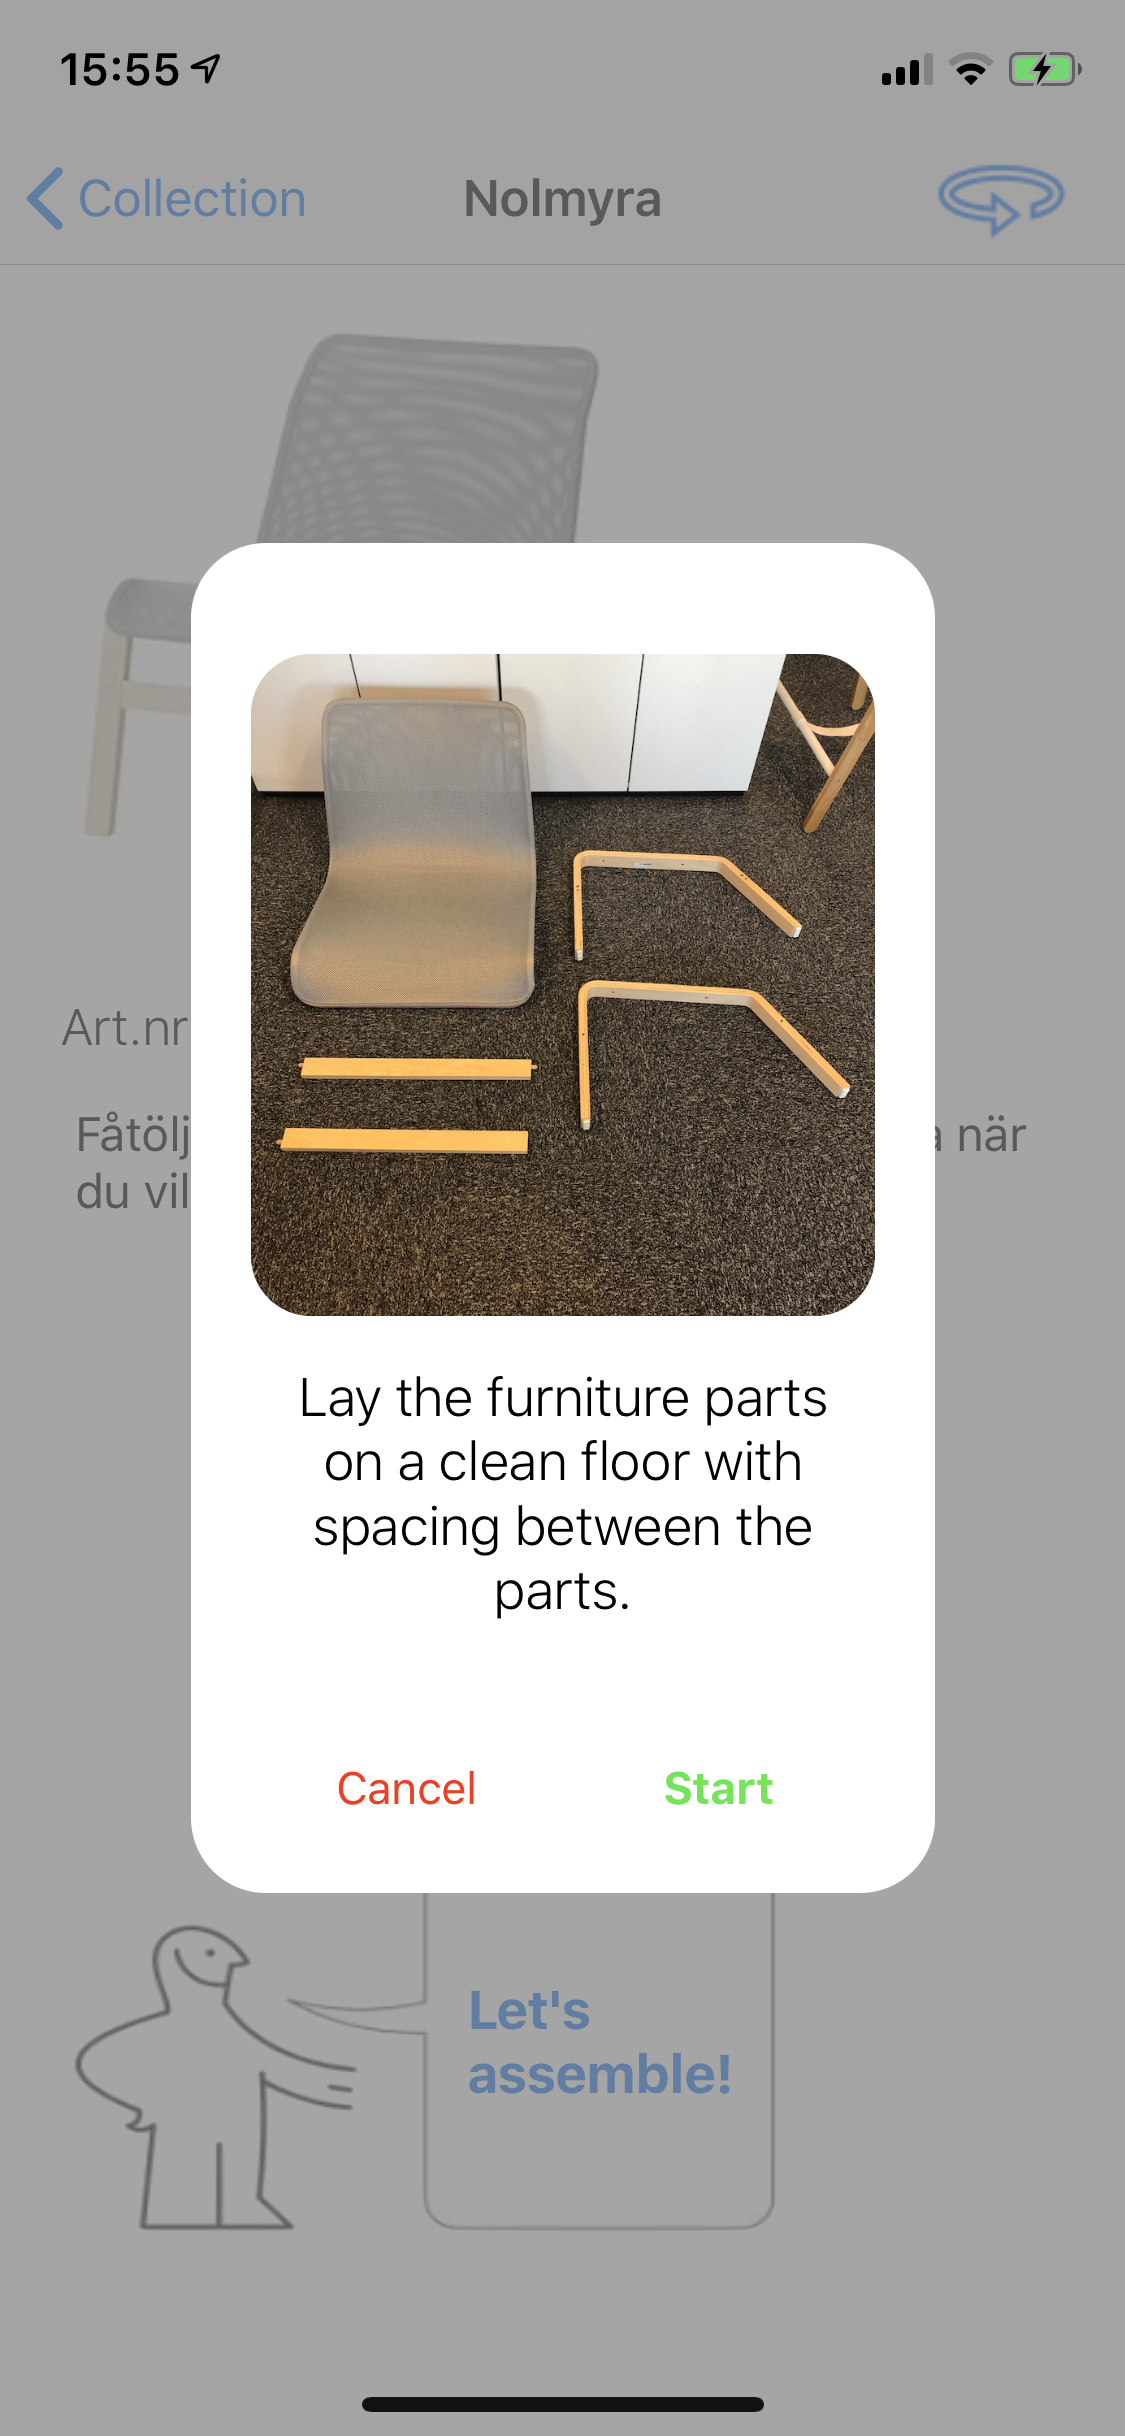
\includegraphics[width = 0.3\textwidth]{./Images/Application3}
\caption{Images from the use of the application when selecting a furniture and right before starting the assembler view.}
\label{fig:applicationSelection}
\end{center}
\end{figure}

\begin{figure}[!hbtp]
\begin{center}
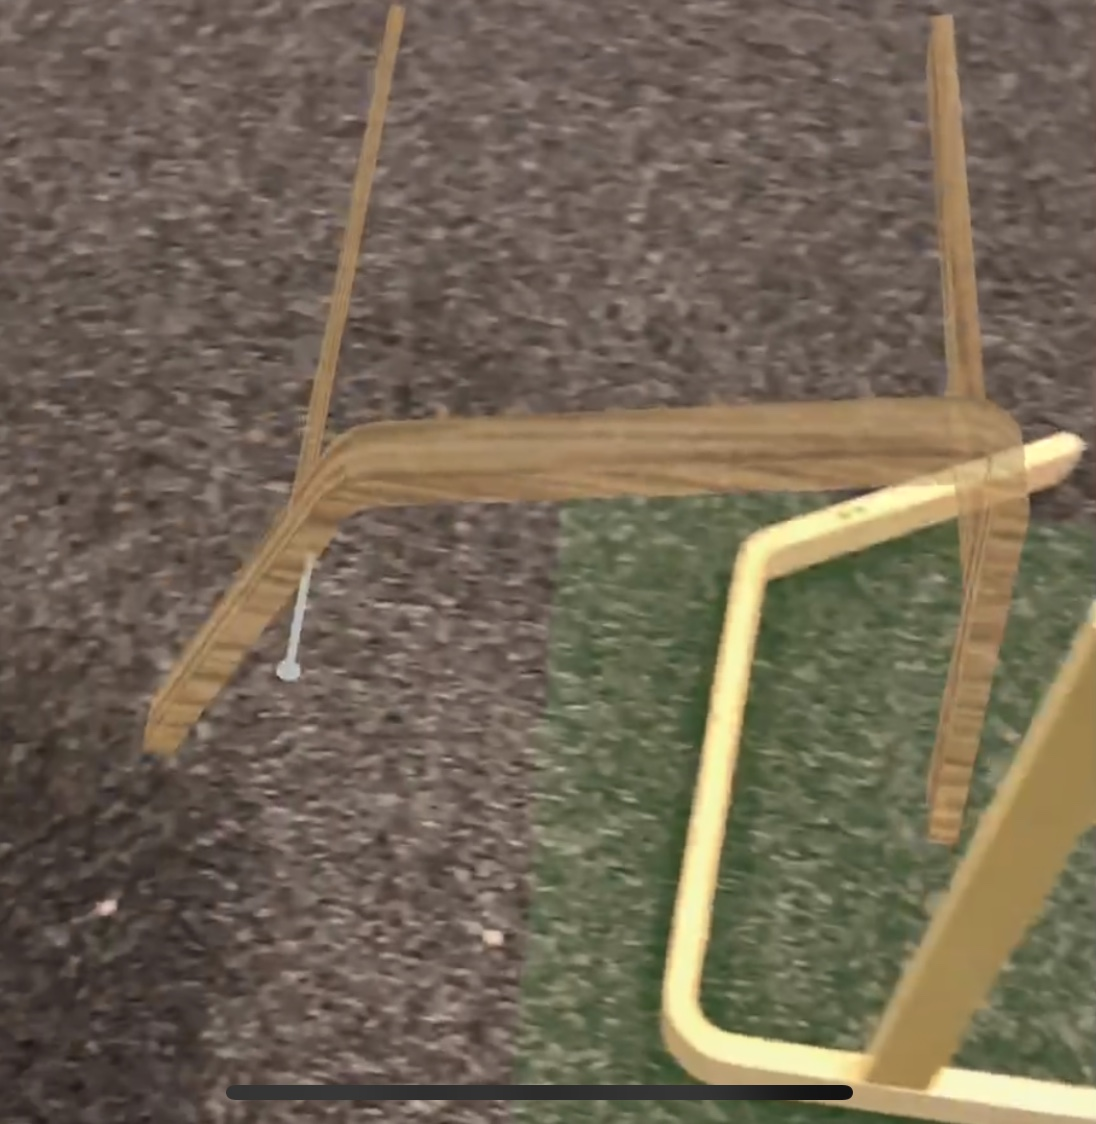
\includegraphics[width = 0.3\textwidth]{./Images/Application4}
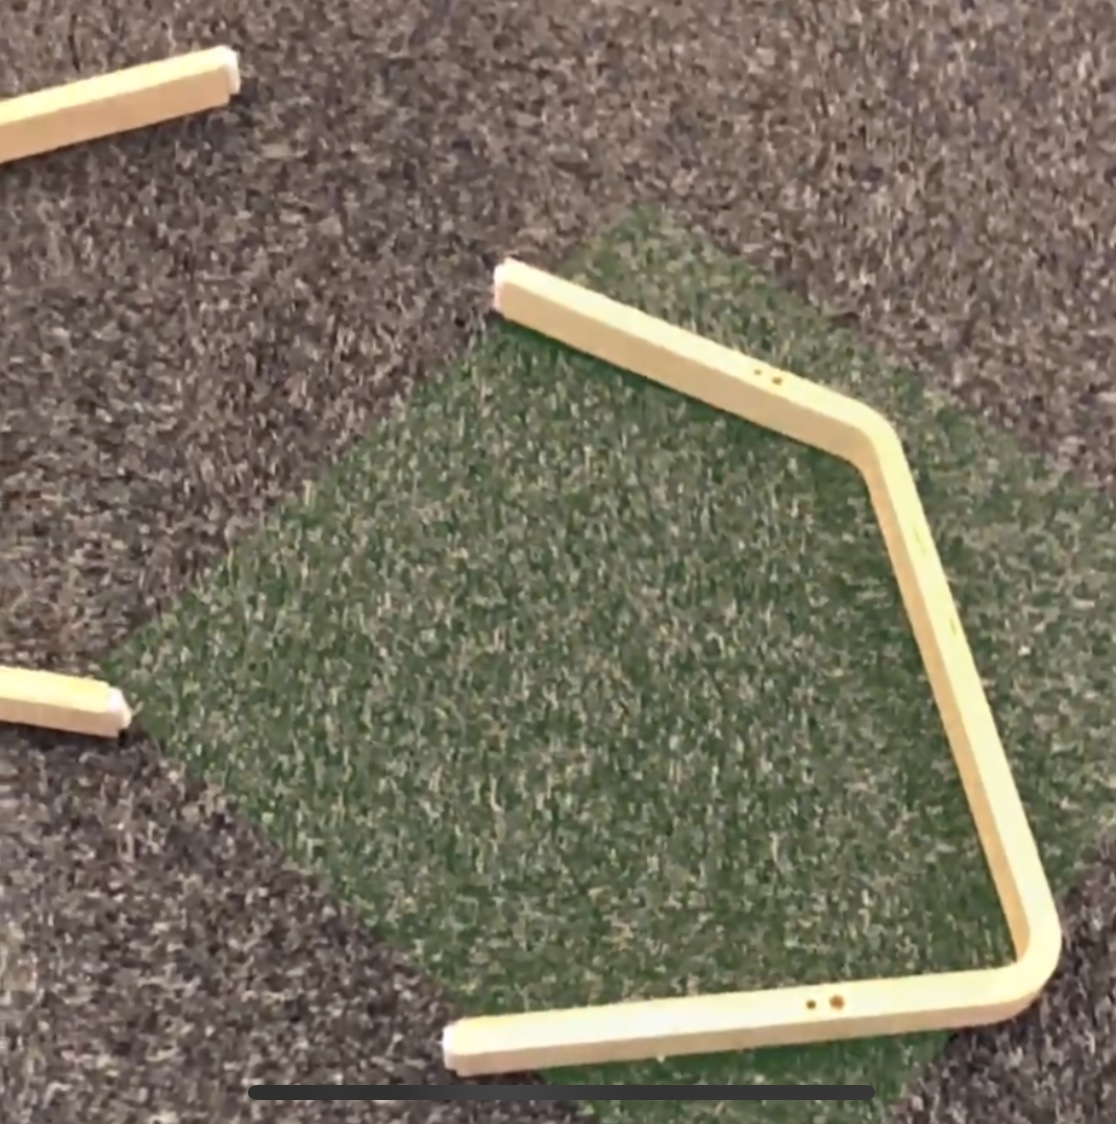
\includegraphics[width = 0.3\textwidth]{./Images/Application5}
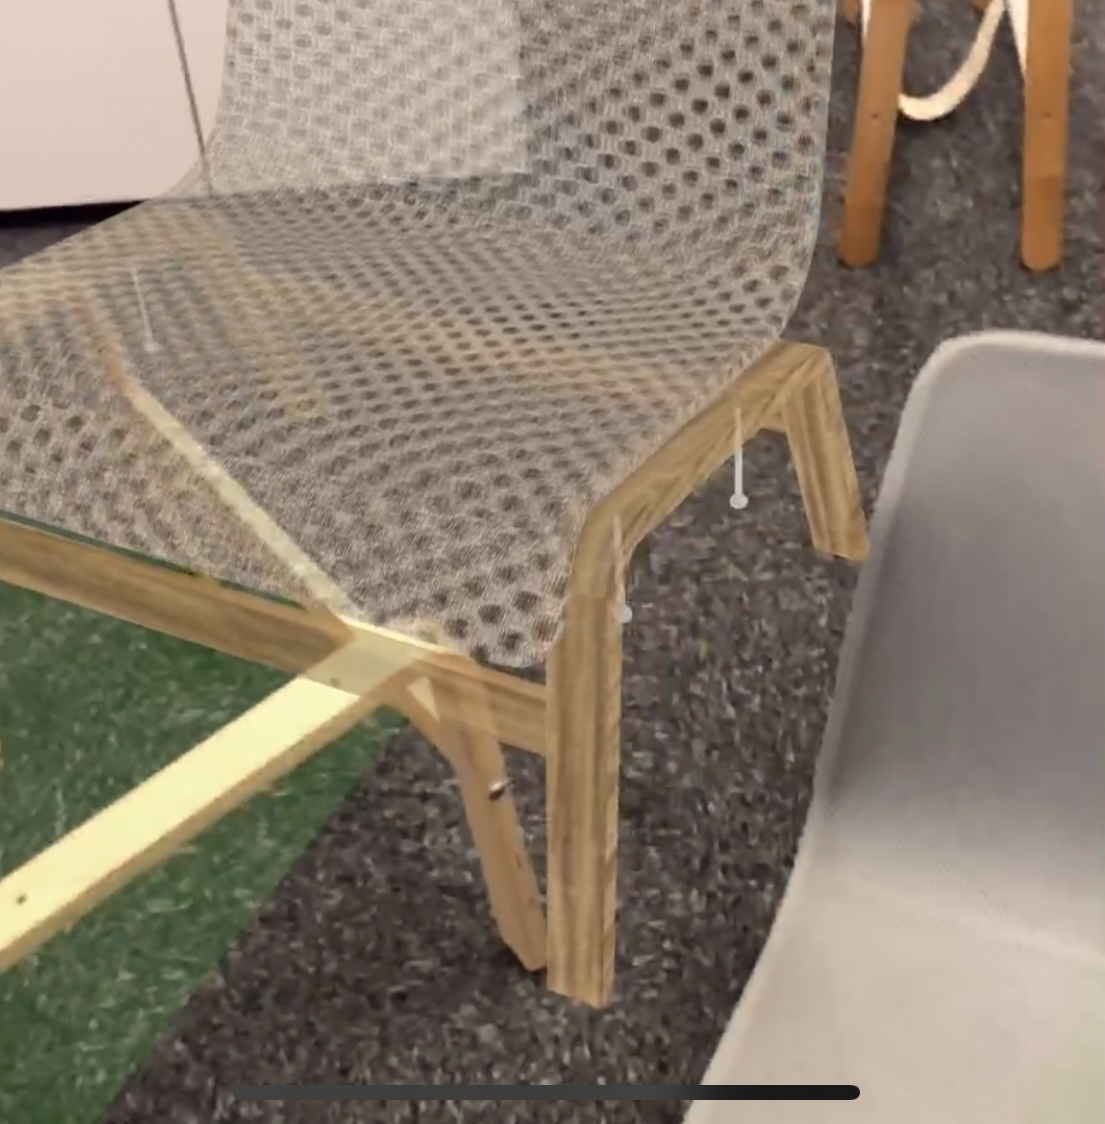
\includegraphics[width = 0.3\textwidth]{./Images/Application6}
\caption{Images from the application when having started the ARScene, finding objects and showing animations when putting them together. The green rectangle on the floor is an indication that the part has been recognized by the application. We call these markings.}
\label{fig:applicationAssembler}
\end{center}
\end{figure}

\section{User Testing}

Evaluating the AR experience is possible on a technical level, to research if the 
combination of AR with object recognition is feasible. This can be done by, for instance,  
making sure the application is running at an acceptable frame rate. However, as this 
report also wants to research into the desirability of this combination of technology, the 
same approach is not as appropriate. What was done was to test the 
application ourselves, as well as get outside evaluations through user tests.

The user tests were set up by having people from the office sign up online to come test our 
application, as well as answering a form afterwards where they answered several 
questions. While the users were doing the tests, they were observed and comments were 
written down, reporting on how they behaved. 

The form asked the participants the following questions:
\begin{itemize}
\item Did you know that you could skip instructions?
\item How easy was it to understand how to get to the next step?
\item How easy was it to understand how the pieces fit together?
\item How easy did you feel the app was to use?
\item Compared to using paper instructions, did the app make it easier to understand how to put together the furniture? ? If not, then why?
\item What potential do you see in this app?
\item General feedback
\item Suggestions of improvement
\item What is your role at Jayway?
\end{itemize}

The answers were then evaluated and the result from this can be read in the result section.



A user survey was done in order to evaluate the performance of the application. By having a multitude of interested people booking time slots for a ten minute testing period, a decent amount of sample data could be gathered and evaluated. Figures \ref{fig:question1} to \ref{fig:question6} show bar charts and pie charts representing the answers gathered from the participants to some of the questions they were asked. 

\begin{figure}[hbtp]
\begin{center}
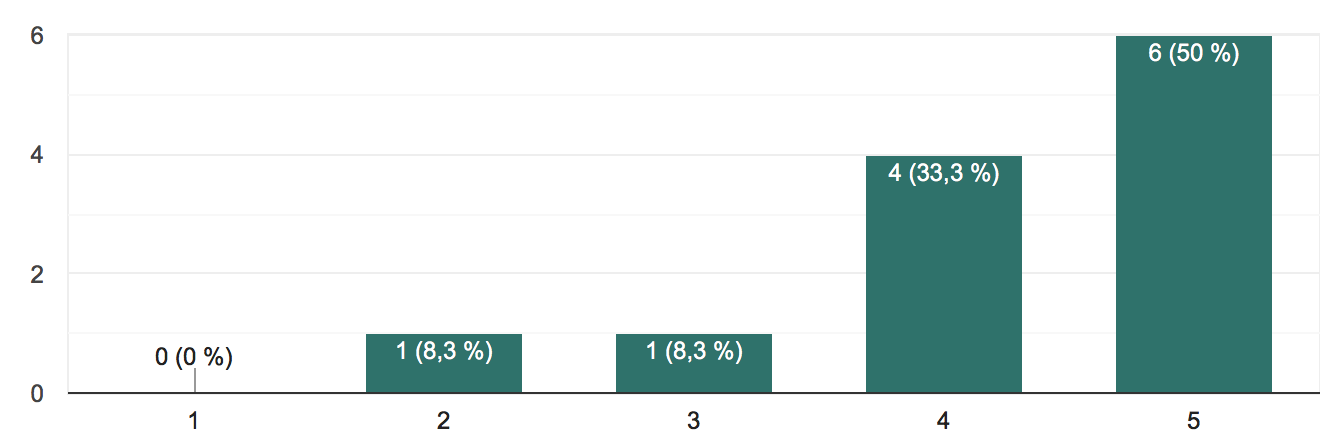
\includegraphics[width = 0.9\textwidth]{./Images/easyToGetToNext.png}
\caption{Results from when users were asked "How easy was it to understand how to get to the next step?"}
\label{fig:question1}
\end{center}
\end{figure}

\begin{figure}[hbtp]
\begin{center}
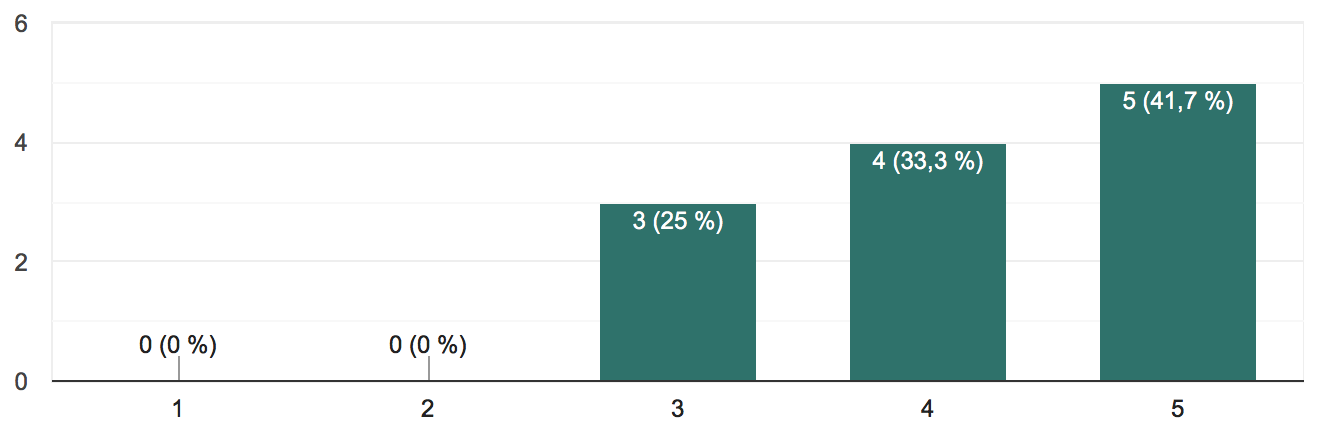
\includegraphics[width = 0.9\textwidth]{./Images/easyToUnderstand.png}
\caption{Results from when users were asked "How easy was it to understand how the pieces fit together?"}
\label{fig:question2}
\end{center}
\end{figure}

\begin{figure}[hbtp]
\begin{center}
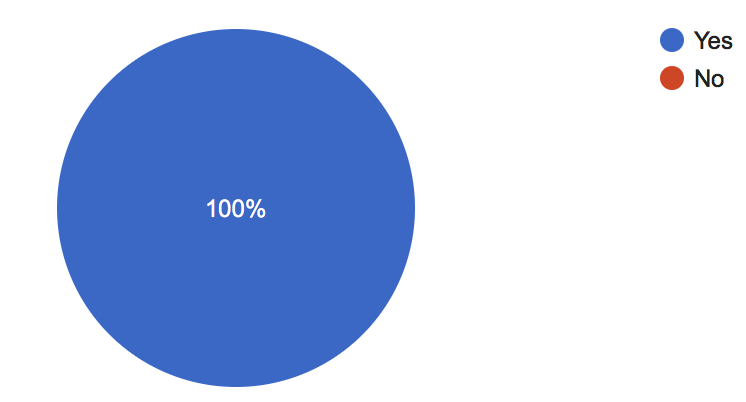
\includegraphics[width = 0.6\textwidth]{./Images/knowToSkip.png}
\caption{Results from when users were asked "Did you know that you could skip instructions?"}
\label{fig:question3}
\end{center}
\end{figure}

\begin{figure}[hbtp]
\begin{center}
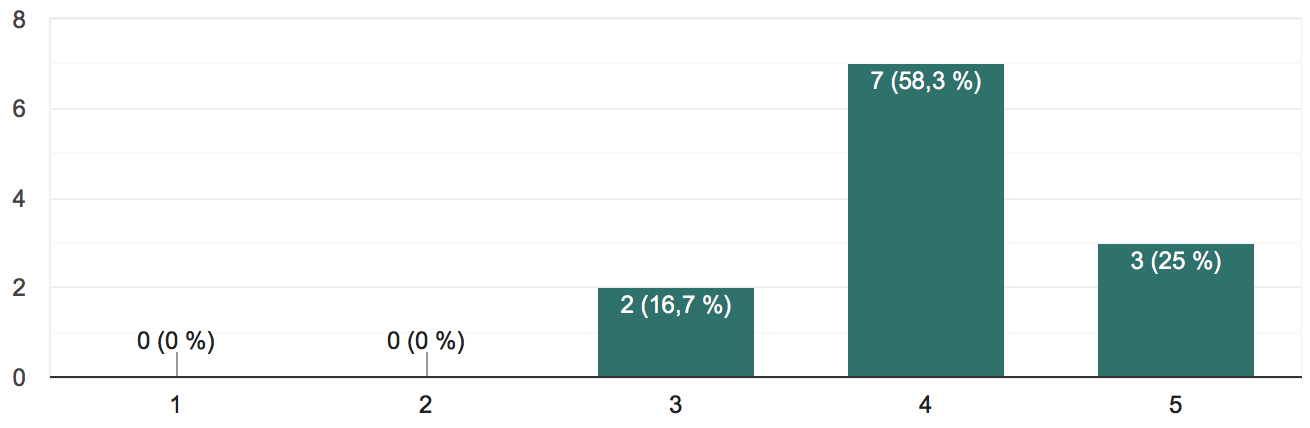
\includegraphics[width = 0.9\textwidth]{./Images/easyToUse.png}
\caption{Results from when users were asked "How easy was it to understand how to get to the next step?"}
\label{fig:question4}
\end{center}
\end{figure}

\begin{figure}[hbtp]
\begin{center}
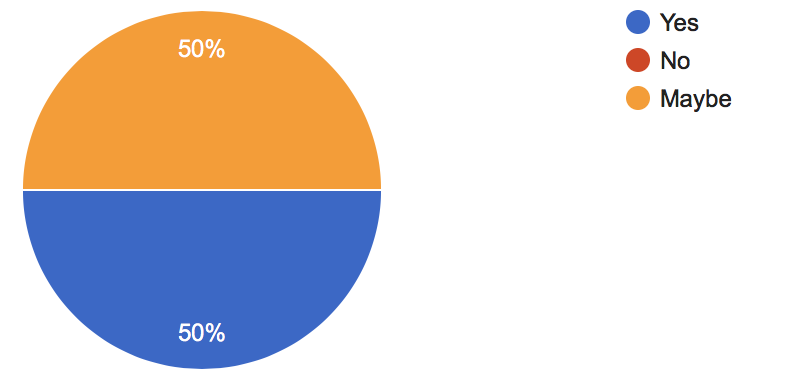
\includegraphics[width = 0.6\textwidth]{./Images/comparedTo.png}
\caption{Results from when users were asked "Compared to using paper instructions, did the app make it easier to understand how to put together the furniture?"}
\label{fig:question5}
\end{center}
\end{figure}

\begin{figure}[hbtp]
\begin{center}
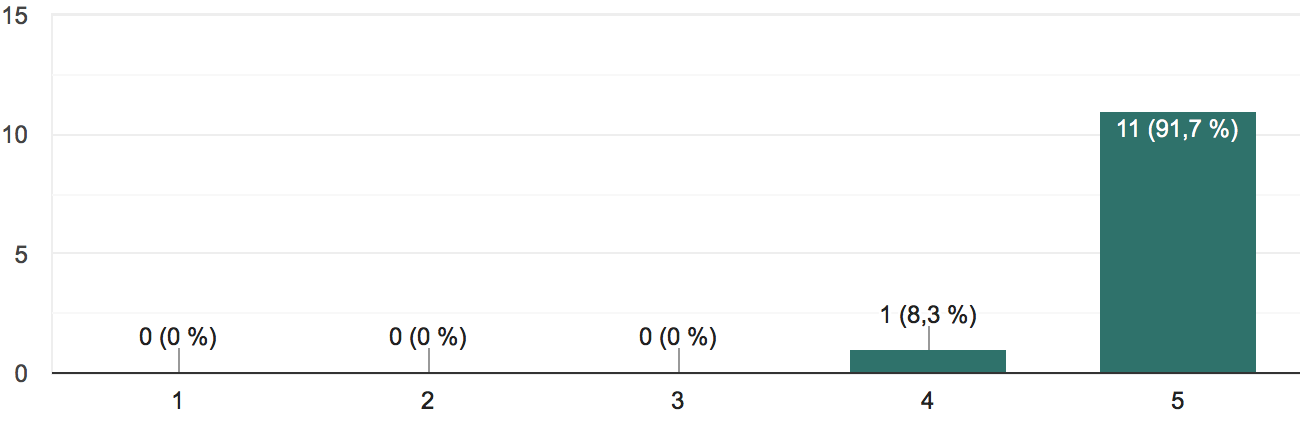
\includegraphics[width = 0.9\textwidth]{./Images/potential.png}
\caption{Results from when users were asked "What potential do you see in this app?"}
\label{fig:question6}
\end{center}
\end{figure}


By collecting the data from the forms, the recorded videos and our own observations we could find some general trends and reach a few conclusions.

What we found was that half of the participants thought it was easier to use our
application to assemble the furniture than using a traditional paper instruction, and none t
thought it was definitively more difficult, as seen in figure \ref{fig:question5}. This could be due to the fact that the piece of furniture we 
chose to train on were quite simple to assemble, relative to other possible furniture. Would be interesting to perform the same task but on a more complicated piece of furniture.

Everyone of the the participants saw that the application good or great potential, see figure \ref{fig:question6}, if it were 
to be improved. This result shows that the use of this technology is mostly desirable, if 
done in a more proper way.

The answers show that most people could understand how to use the application and 
could intuitively start up the application and start the assembly process without outside 
help, figure \ref{fig:question1}, \ref{fig:question2} \& \ref{fig:question4}. In some cases we noticed that people were a bit confused with the augmented reality 
interface. Several participants had a hard time understanding the purpose of the green 
rectangles that were rendered around a found object in the scene. Mostly because the 
rectangles were significantly larger than the object itself, hence, it often overlaps with 
other objects on the floor.

The hassle of having to put the phone down in between looking at the animation and 
actually assembling the furniture parts was also brought up. Some of the participants had 
to pick up the phone several times during certain steps to make sure they were executing 
the task in the correct manner.

At times, some participants were getting confused because the application could not find 
the correct parts. This happened because of several reasons. One being that they had 
accidentally skipped an instruction, thus the application were looking for model parts that 
had not yet been assembled. Another reason being that the machine learning model were 
inconsistent at times and could not identify certain in the orientation it was currently in. It 
also happened when the users did not perform 
the first task given by the application, being that they had to make sure that the parts were 
laying on the floor and not overlapping each other. A solution to these problems could be 
to give the users a more clarified and more intuitive set of instructions such that the user 
don't accidentally skip an important instruction. Another solution is to retrain the machine 
learning model to be able to identify the parts in more orientations. 

The user test was performed in the Jayway offices on people with background in 
technology, where most participants were developers or designers. Due to this, the result 
could be skewed, since people with similar background have a tendency to understand 
each others intent. The same test would have to be performed on actual end users with a 
more varied background to see if it would match the results we've gathered.
\newpage